\model{POGIL Research}

\textit{Process-Oriented Guided Inquiry Learning} (see \href{https://pogil.org/}{pogil.org}) is a student-centered, team-learning instructional strategy and philosophy developed through research on how students learn best.
The following two figures are from peer-reviewed articles published in education journals.

% images from Chapter 8 of http://dx.doi.org/10.7936/K7PN93HC

\vspace{1em}
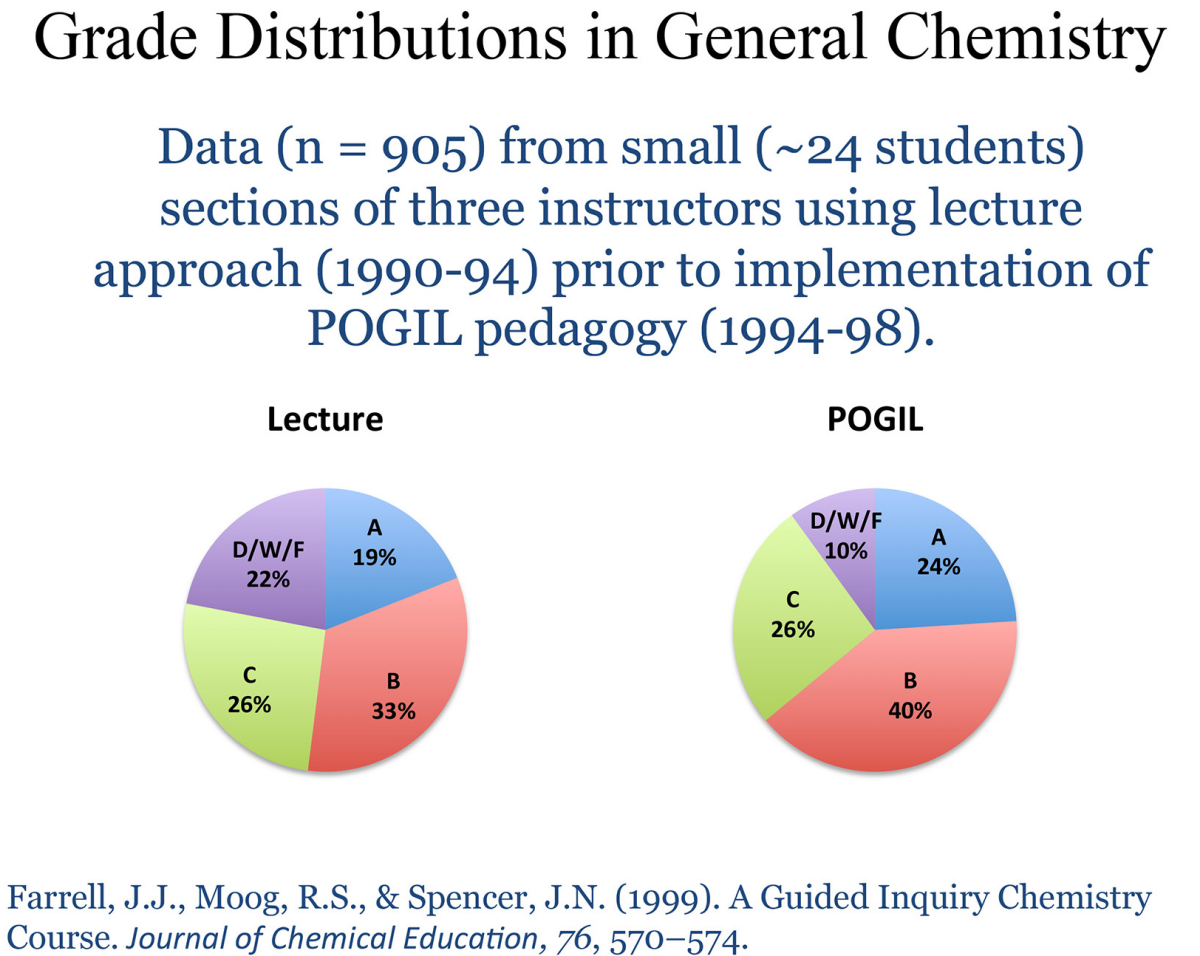
\includegraphics[width=0.47\linewidth]{pogil-grades.png}
\hfill
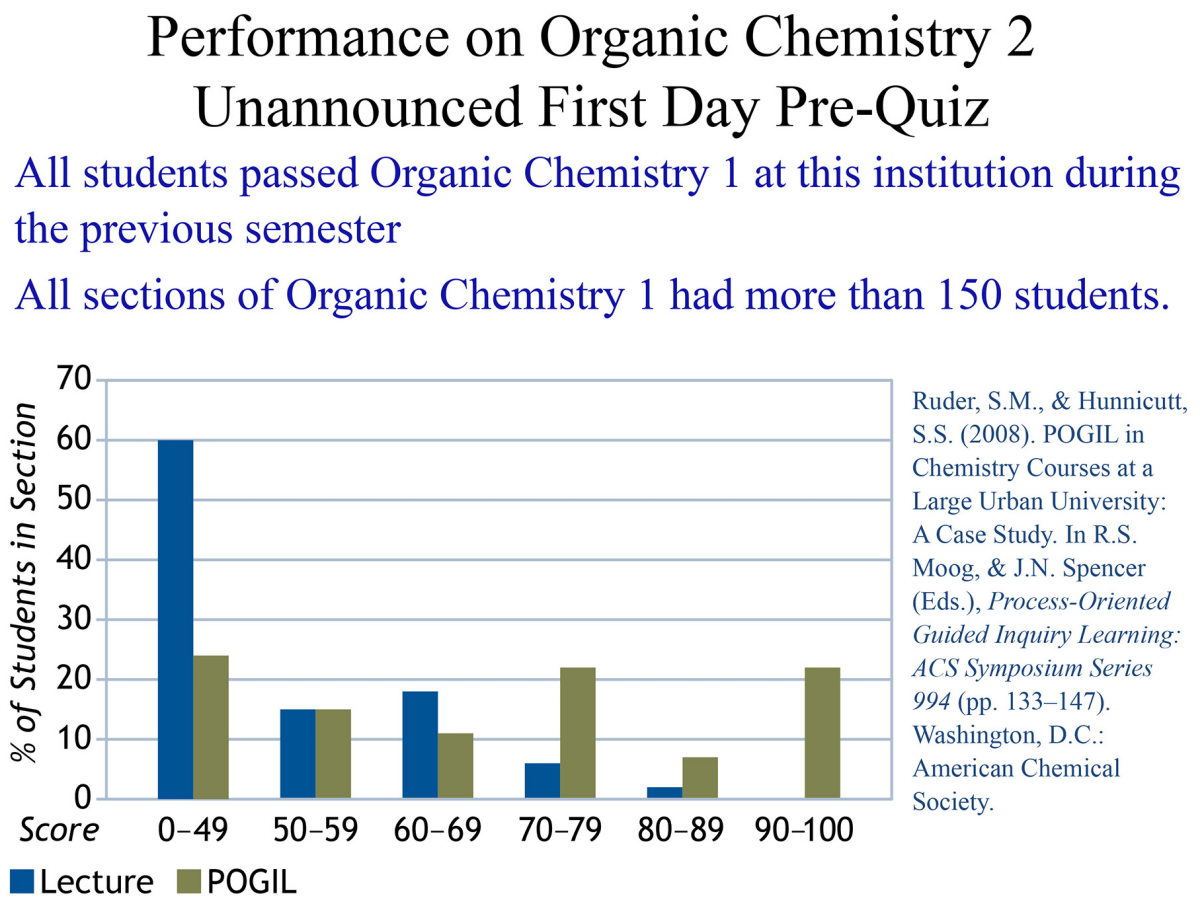
\includegraphics[width=0.50\linewidth]{pogil-prequiz.png}


\quest{10 min}


\Q How large were the classes at each of the universities shown above?

\begin{answer}[2em]
The left university had classes of about 24, and the right had over 150 students/section.
\end{answer}


\Q What are the measures of performance shown in each of the figures?

\begin{answer}[2em]
The left figure shows grade distributions, and the right figure shows pre-quiz scores.
\end{answer}


\Q What does the figure on the left suggest about POGIL's impact on student success?

\begin{answer}[6em]
``Students in courses employing a POGIL instructional strategy achieved a significantly higher success rate (defined as receiving an A, B, or C in the course, as compared to a D, F or withdrawal) than students who had been taught by the same instructors in previous years using a more traditional lecture-oriented approach.
In both cases, the students were in classes of about 24 students each, and similar exams were used for both groups of students.'' (Moog 2014)
\end{answer}


\Q What does the figure on the right suggest about students' retention of knowledge?

\begin{answer}[6em]
``A majority of the students (60\%) in the lecture section scored below 50 percent on the quiz, and none of the students achieved a score above 90 percent.
Less than five percent scored above 80 percent.
In contrast, fewer than a a quarter of the students from the POGIL section scored below 50 percent on this quiz, and about 30 percent of the students scored above 80 percent, with over one-fifth of the POGIL
students scoring above 90 percent.'' (Moog 2014)
\end{answer}
